\section{Dossier de spécifications}

\par À l’issue de la première réunion avec Mr Stéphane Vialle (encadrant de projet), cahier des charges, déroulement du projet, éventuelles difficultés et objectif du projet développement ont été établis. Ce dernier point consiste à nous enseigner à :
\begin{itemize}
\item formaliser un cahier des charges
\item décrire un projet sous forme UML (diagramme de classe, séquence, use case)
\item réaliser un plan de test
\item réaliser une documentation et une architecture logicielle (user guide)
\item coder une interface graphique (présence d’héritage)
\item travailler sur des fichiers I/O
\end{itemize}

\par Ainsi l’architecture globale du projet est donnée à la figure ci-dessous. L’idée est d’agréger une couche logicielle à l’environnement OAR qui permet de gérer les ressources physiques du cluster et qui est accessible via le shell.  Pour de amples informations sur OAR et les commandes shell nécessaires afin de se connecter et d’allouer des nœuds de calcul, vous vous référerez aux parties correspondantes.

\par Le but dans tout ceci est d’allouer des nœuds dont la description est décrite au sein d’un fichier .txt et qui sera présenté à l’utilisateur.
\begin{figure}[h!]
  \centering
  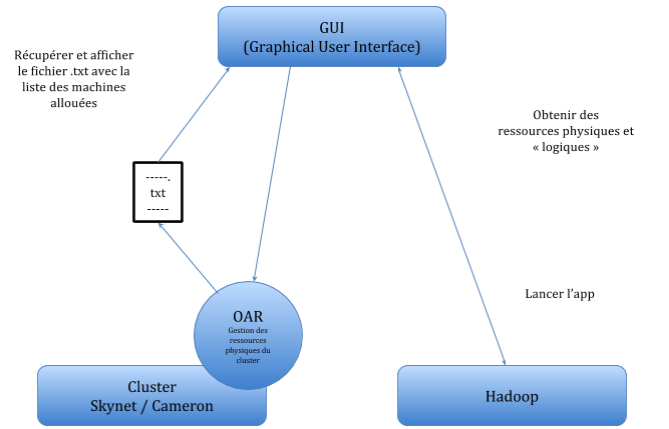
\includegraphics[width=14cm]{images/schema_global.png}
  \caption{Schéma global de fonctionnement de l'application}
  \label{fig:schema_global}
\end{figure}

\par Il s’agit ensuite d’utiliser cette même GUI afin de lancer des applications Hadoop. Afin de se familiariser avec cet environnement, on codera une application permettant de réaliser du Data Mining sur un document texte : autrement dit, de chercher un certain mot et son occurrence dans le document fourni. C’est ce qui fera l’objet de la deuxième partie du projet.
Par ailleurs, dans le cadre du projet, les accès serveurs nous ont été autorisés sur nos comptes Supélec.

\subsection{Le diagramme Use case}
\label{sec:le-diagramme-use}

La figure \ref{fig:use_case} donne le diagramme use case du projet. L’objectif final de l’utilisateur étant de créer un job (allocation de nœuds) afin d’exécuter un script, il devra au préalable s’identifier auprès des serveurs GHOME et TERM2.
\begin{itemize}
\item On peut ainsi répertorier plusieurs scénarios
\item S’identifier
\item Créer un job (Allocation de nœuds)
\item Tuer le job
\item Exécuter un script (Hadoop)
\end{itemize}

\begin{figure}[h!]
  \centering
  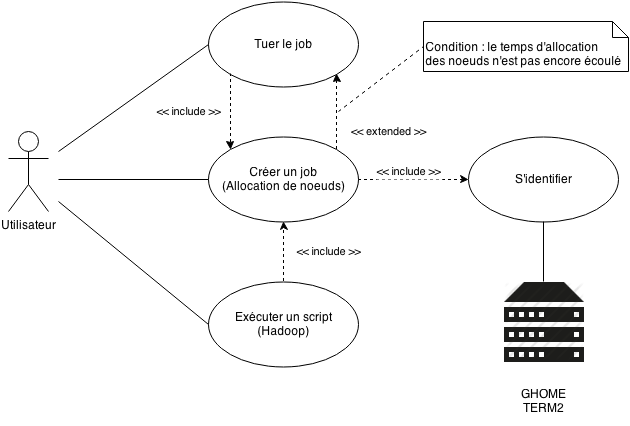
\includegraphics[width=14cm]{images/use_case.png}
  \caption{Use case}
  \label{fig:use_case}
\end{figure}

\paragraph{Scénario «S’identifier»}
L’identification de l’utilisateur passe d’abord par l’identification auprès du serveur GHOME puis de TERM2. S’identifier auprès de GHOME est nécessaire si l’utilisateur se trouve à l’extérieur du réseau Supélec. Dans le cas contraire il suffit de s’identifier uniquement auprès de TERM2. Cependant, bien que l’utilisateur se situe au sein du réseau Supélec, lui demander de s’identifier auprès de GHOME ne gêne pas le cours de l’identification. Par souci de praticité, l’utilisateur s’identifiera toujours auprès de GHOME puis de TERM2.
Cette étape consiste à vérifier que le nom ainsi que le mot de passe de l’utilisateur sont valides.

\paragraph{Scénario «Créer un job (Allocation de nœuds)»}
\label{sec:scenario-creer-un}
Après s’être identifié, l’utilisateur sera en mesure de créer un job, i.e. d’allouer des nœuds de calcul. Il renseignera donc le nombre de nœuds souhaités ainsi que le temps d’allocation. Deux cas de figure se présentent par la suite.
Après la création d’un job, si le temps d’allocation est écoulé, alors le job meurt automatique. Dans le cas contraire, l’utilisateur pourra interagir avec la GUI pour mettre fin à son job afin d’en créer un nouveau.

\paragraph{Scénario «Tuer le job»}
\label{sec:scenario-tuer-le}
Comme mentionné précédemment, ce scénario n’est possible que lorsqu’un job a été créé et donc que l’utilisateur s’est connecté au serveur. 

\paragraph{Scénario «Exécuter un script (Hadoop)»}
\label{sec:scenario-executer-un}
Ce scénario sera abordé dans la deuxième partie du projet se déroulant au cours de la séquence 8.


\subsection{Cahier des charges}
\label{sec:cahier-des-charges}

\par Le cahier des charges s’articule en trois parties.

\paragraph{Points essentiels}
\label{sec:points-essentiels}

\par Après analyse du problème posé, trois points essentiels du projet ont été retenus. D’abord nous créerons une IU de connexion aux serveurs à travers laquelle on spécifiera le nom de la machine, le nom utilisateur et son mot de passe.
Ensuite, on créera une deuxième IU d’allocation des nœuds ou sont spécifiés le nombre de nœuds, leur temps d’allocation ainsi que le mode d’allocation (on choisit par défaut le mode interactif).
Enfin, un fichier .txt contenant la description des nœuds alloués devra être créé.

\begin{figure}[h!]
  \centering
  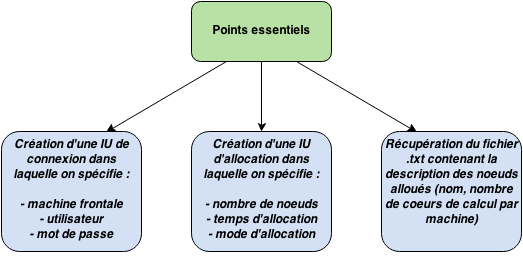
\includegraphics[width=14cm]{images/points_essentiels.png}
  \caption{Points essentiels}
  \label{fig:pts_essentiels}
\end{figure}


\paragraph{Points souhaités}
\label{sec:points-souhaites}

\par Parmi les options fortement souhaitées, l’IU d’allocation devra comporter une zone de texte où sera affiché le temps d’allocation des nœuds en temps réel ainsi que les noms des machines allouées. En outre, le fichier .txt devra être affiché dans cette zone de texte.

\begin{figure}[h!]
  \centering
  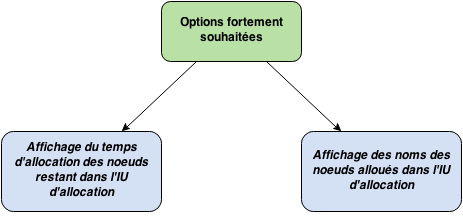
\includegraphics[width=14cm]{images/points_souhaites.png}
  \caption{Points souhaités}
  \label{fig:pts_souhaites}
\end{figure}

\paragraph{Points optionnels}
\label{sec:points-optionnels}

\par Nous avons retenu trois développements optionnels. Leur réalisation est conditionnée par l’état d’avancement du projet (priorité aux points essentiels et aux options fortement souhaitées) et de leur faisabilité technique.
\par Le premier consiste à avoir un état des lieux du serveur, i.e. à recenser les ressources physiques disponibles lors de la connexion. L’idée étant dans une deuxième partie de donner à l’utilisateur la possibilité de choisir entre les différents clusters les machines avec lesquelles il souhaite travailler. En effet, selon que l’on se trouve sur le cluster Skynet, Cameron ou InterCel, les machines ne possèdent pas les mêmes puissances de calcul.
\par Troisièmement, dans le souci de rendre l’expérience utilisateur la plus agréable possible, un design épuré serait fort appréciable. Bien entendu, ce point sera abordé uniquement si tous les précédents points sont opérationnels.

\begin{figure}[h!]
  \centering
  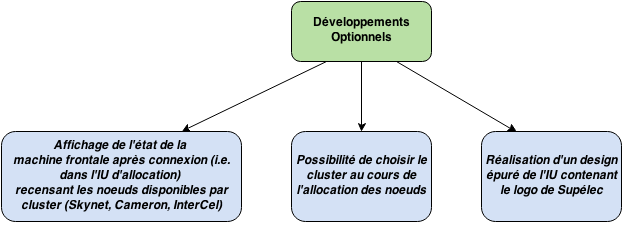
\includegraphics[width=14cm]{images/points_optionnels.png}
  \caption{Points optionnels}
  \label{fig:pts_optionnels}
\end{figure}



%%% Local Variables: 
%%% mode: latex
%%% TeX-master: "CompteRendu"
%%% End: 
